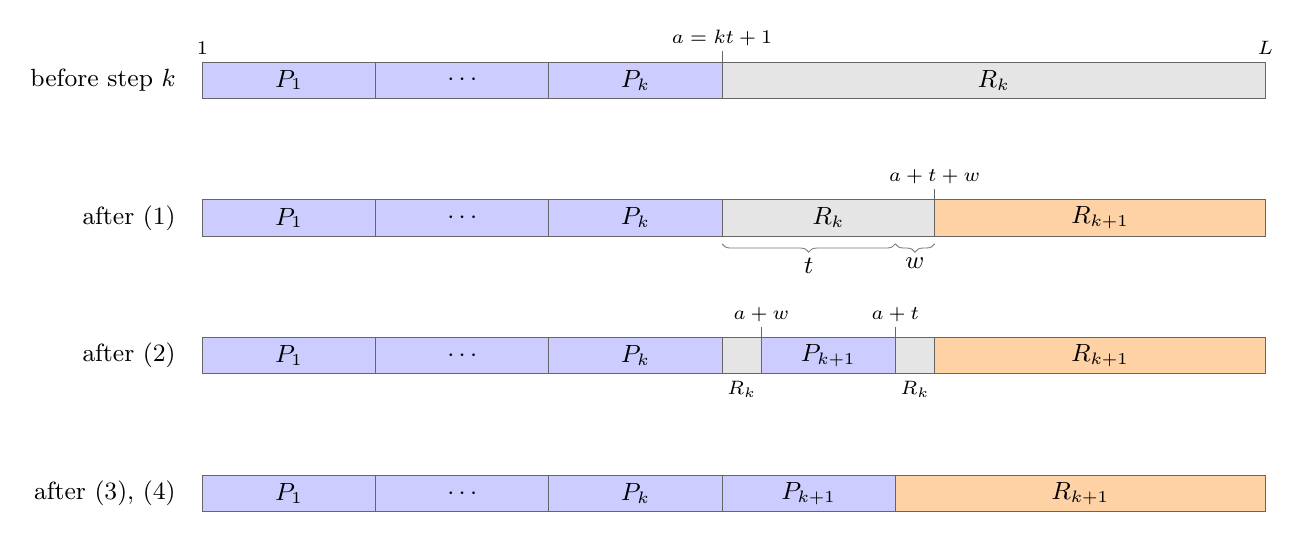
\begin{tikzpicture}[x=1cm, y=1cm, line width=0.3pt,
    lab/.style={font=\small, inner sep=1pt},
    name/.style={font=\scriptsize, text=black!55, inner sep=1pt},
    coord/.style={font=\scriptsize, inner sep=1pt},
    seg/.style={draw=black!60, line width=0.3pt},
    P/.style={seg, fill=blue!20},
    Rk/.style={seg, fill=black!10},
    Rn/.style={seg, fill=orange!35},
    brace/.style={decorate, decoration={brace, mirror, amplitude=3pt}}]
  \def\t{2.2}\def\w{0.5}\def\L{13.5}
  \def\a{6.6}      % a = k t + 1, the first site of block k+1 (3 t)
  \def\h{0.46}     % bar height
  \def\dy{1.75}    % row spacing
  \begin{scope}[yshift=0cm]
    \node[lab, anchor=east] at (-0.3, 0.5*\h) {before step \(k\)};
    \fill[P] (0, 0) rectangle (\t, \h);
    \fill[P] (\t, 0) rectangle (2*\t, \h);
    \fill[P] (2*\t, 0) rectangle (\a, \h);
    \fill[Rk] (\a, 0) rectangle (\L, \h);
    \node[lab] at (0.5*\t, 0.5*\h) {\(P_1\)};
    \node[lab] at (1.5*\t, 0.5*\h) {\(\cdots\)};
    \node[lab] at (2.5*\t, 0.5*\h) {\(P_k\)};
    \node[lab] at ({0.5*(\a+\L)}, 0.5*\h) {\(R_k\)};
    \node[coord, anchor=south] at (0, \h+0.05) {\(1\)};
    \node[coord, anchor=south] at (\L, \h+0.05) {\(L\)};
    \draw[black!60] (\a, \h) -- (\a, \h+0.14);
    \node[coord, anchor=south] at (\a, \h+0.16) {\(a=kt+1\)};
  \end{scope}
  \begin{scope}[yshift=-\dy cm]
    \node[lab, anchor=east] at (-0.3, 0.5*\h) {after (1)};
    \fill[P] (0, 0) rectangle (\t, \h);
    \fill[P] (\t, 0) rectangle (2*\t, \h);
    \fill[P] (2*\t, 0) rectangle (\a, \h);
    \fill[Rk] (\a, 0) rectangle (\a+\t+\w, \h);
    \fill[Rn] (\a+\t+\w, 0) rectangle (\L, \h);
    \node[lab] at (0.5*\t, 0.5*\h) {\(P_1\)};
    \node[lab] at (1.5*\t, 0.5*\h) {\(\cdots\)};
    \node[lab] at (2.5*\t, 0.5*\h) {\(P_k\)};
    \node[lab] at ({\a+0.5*(\t+\w)}, 0.5*\h) {\(R_k\)};
    \node[lab] at ({0.5*(\a+\t+\w+\L)}, 0.5*\h) {\(R_{k+1}\)};
    \draw[black!60] (\a+\t+\w, \h) -- (\a+\t+\w, \h+0.14);
    \node[coord, anchor=south] at (\a+\t+\w, \h+0.16) {\(a+t+w\)};
    \draw[brace, black!55] (\a, -0.1) -- (\a+\t, -0.1)
      node[lab, midway, below=4pt, text=black] {\(t\)};
    \draw[brace, black!55] (\a+\t, -0.1) -- (\a+\t+\w, -0.1)
      node[lab, midway, below=4pt, text=black] {\(w\)};
  \end{scope}
  \begin{scope}[yshift=-2*\dy cm]
    \node[lab, anchor=east] at (-0.3, 0.5*\h) {after (2)};
    \fill[P] (0, 0) rectangle (\t, \h);
    \fill[P] (\t, 0) rectangle (2*\t, \h);
    \fill[P] (2*\t, 0) rectangle (\a, \h);
    \fill[Rk] (\a, 0) rectangle (\a+\w, \h);
    \fill[P] (\a+\w, 0) rectangle (\a+\t, \h);
    \fill[Rk] (\a+\t, 0) rectangle (\a+\t+\w, \h);
    \fill[Rn] (\a+\t+\w, 0) rectangle (\L, \h);
    \node[lab] at (0.5*\t, 0.5*\h) {\(P_1\)};
    \node[lab] at (1.5*\t, 0.5*\h) {\(\cdots\)};
    \node[lab] at (2.5*\t, 0.5*\h) {\(P_k\)};
    \node[lab] at ({\a+0.5*(\t+\w)}, 0.5*\h) {\(P_{k+1}\)};
    \node[lab] at ({0.5*(\a+\t+\w+\L)}, 0.5*\h) {\(R_{k+1}\)};
    \node[coord, anchor=north] at (\a+0.5*\w, -0.06) {\(R_k\)};
    \node[coord, anchor=north] at (\a+\t+0.5*\w, -0.06) {\(R_k\)};
    \draw[black!60] (\a+\w, \h) -- (\a+\w, \h+0.14);
    \node[coord, anchor=south] at (\a+\w, \h+0.16) {\(a+w\)};
    \draw[black!60] (\a+\t, \h) -- (\a+\t, \h+0.14);
    \node[coord, anchor=south] at (\a+\t, \h+0.16) {\(a+t\)};
  \end{scope}
  \begin{scope}[yshift=-3*\dy cm]
    \node[lab, anchor=east] at (-0.3, 0.5*\h) {after (3), (4)};
    \fill[P] (0, 0) rectangle (\t, \h);
    \fill[P] (\t, 0) rectangle (2*\t, \h);
    \fill[P] (2*\t, 0) rectangle (\a, \h);
    \fill[P] (\a, 0) rectangle (\a+\t, \h);
    \fill[Rn] (\a+\t, 0) rectangle (\L, \h);
    \node[lab] at (0.5*\t, 0.5*\h) {\(P_1\)};
    \node[lab] at (1.5*\t, 0.5*\h) {\(\cdots\)};
    \node[lab] at (2.5*\t, 0.5*\h) {\(P_k\)};
    \node[lab] at (\a+0.5*\t, 0.5*\h) {\(P_{k+1}\)};
    \node[lab] at ({0.5*(\a+\t+\L)}, 0.5*\h) {\(R_{k+1}\)};
  \end{scope}
\end{tikzpicture}
